\ProvidesFile{ap-accessibility.tex}[2024-03-15 accessibility appendix]

\begin{VerbatimOut}{z.out}
\chapter{ACCESSIBILITY}
\ix{accessibility//Accessibility appendix}
\end{VerbatimOut}

\MyIO


\begin{VerbatimOut}{z.out}

Accessibility is the design of products,
devices,
services,
vehicles,
or environments
so as to be usable by people with disabilities.
\cite{wikipedia-accessibility}
\end{VerbatimOut}

\MyIO


\begin{VerbatimOut}{z.out}


\section{Color}

Color vision deficiency (CVD) affects more than 4\% of the population
and leads to a different visual perception of colors.
The cividis%
\ix{cividis colormap}
colormap is optimal
for viewing
by those with or without CVD
\cite{nunez2018}.
The
\citetitle{senn2022}
\cite{senn2022}
and
\citetitle{senn2022b}
\cite{senn2022b}
contain the Mathematica code used to produce this cividis example:\\[\baselineskip]
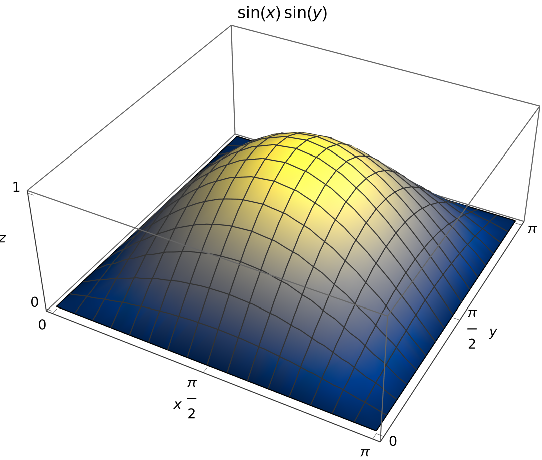
\includegraphics{gr-cividis.pdf}
\end{VerbatimOut}

Please use the cividis colormap for accessibility
unless there is a good reason not to.
\MyIO


\begin{VerbatimOut}{z.out}


\section{PDF file}

The \LaTeXLogo\ Project
\cite{thelatexproject2023}
is working on making tagged
and accessible PDF files with \LaTeXLogo\ %
\cite{mittlebach2022}.
It was not finished as of December 23, 2022.
\end{VerbatimOut}

\MyIO
